\documentclass{beamer}

\usepackage[utf8]{inputenc}
\usepackage[T2A]{fontenc}
\usepackage[russian]{babel}
\usepackage{url}

\usepackage{amsmath}
\usepackage{tikz}
\usepackage{graphicx}
\usepackage{svg}

\usetheme{Madrid}

\defbeamertemplate*{title page}{customized}[1][]
{
    \begin{center}
        \usebeamerfont{title}
        \inserttitle
        \par
    \end{center}
    \bigskip
    \hfill
    \hbox{
        \usebeamerfont{author}
        \begin{tabular}{ll}
            Студент: & Суркис Антон Игоревич \\
            Научный руководитель: & Попов Иван Александрович \\
        \end{tabular}
    }
    \par
    \begin{center}
        \usebeamerfont{date}
        \insertdate
        \par
    \end{center}
}

\title[Ограничения Nanite]{Исследование ограничений процедурного кластерного видозависимого лоддирования в современных компьютерных играх}
\author{Антон Суркис}

\begin{document}
    \maketitle

    \begin{frame}{Введение}
        \begin{itemize}
            \item В современных компьютерных играх для реалистичной графики используют высокодетализированные модели объектов
            \item Отрисовывать все детали всех объектов на экране очень долго
            \item Нужна реакция на ввод в реальном времени
        \end{itemize}
    \end{frame}

    \begin{frame}{Лоды}
        \begin{itemize}
            \item Классическое решение --- уровни детализации, ,,лоды``
            \item Лоды создаются вручную, это дорого
            \item Лоды сложно применять на больших объектах (зданиях, скалах)
        \end{itemize}
        \begin{center}
            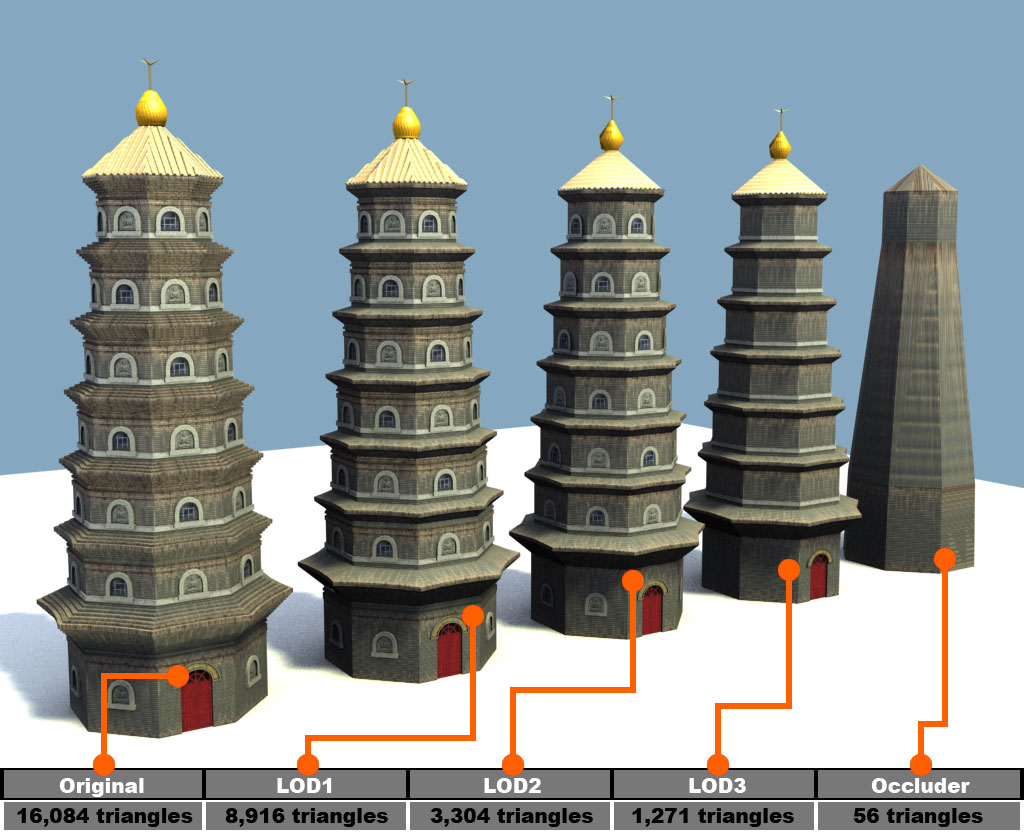
\includegraphics[height=.625\textheight]{lod.jpg}
        \end{center}
    \end{frame}

    \begin{frame}{Альтернативы лодам}
        \begin{itemize}
            \item Clipmaps --- только для ландшафта
            \item Sparse Voxel Octrees от id Software --- неточен, требует много памяти
            \item Nanite от Epic Games --- лучшее известное решение:
            \begin{itemize}
                \item Не нужна ручная обработка
                \item Хорошо работает на больших объектах
                \item Максимальная детализация, на которую хватает разрешения экрана
            \end{itemize}

            \alert{Но за 4 года его так и не скопировали}
        \end{itemize}
    \end{frame}

    \begin{frame}{Цели и задачи}
        \textbf{Цель работы:}
        исследовать ограничения динамической кластерной детализации,
        существенные для компании-разработчика игр.

        \bigskip

        \textbf{Задачи:}
        \begin{itemize}
            \item Изучить механизм работы Nanite
            \item Реализовать упрощённую систему динамической кластерной детализации
            \item Определить проблемы, которые надо решать при реализации полной версии
            \item Определить принципиальные ограничения технологии
            % \item Сравнить с ,,монолитной`` детализацией
        \end{itemize}
    \end{frame}

    \begin{frame}{Nanite}
        Общий механизм работы Nanite\footnote{\url{https://advances.realtimerendering.com/s2021/Karis_Nanite_SIGGRAPH_Advances_2021_final.pdf}} состоит из двух этапов:
        \begin{itemize}
            \item Предподсчёт --- преобразование модели
            \item Непосредственно отрисовка
        \end{itemize}
    \end{frame}

    \begin{frame}{Nanite: предподсчёт}
        \begin{itemize}
            \item Меш разбивается на мешлеты
            \item Строится граф, в котором мешлеты --- вершины
            \item Граф похож на дерево
            \item Исходные мешлеты --- листья
            \item \alert{Свойство графа: родитель менее детализирован, чем ребёнок, с любого ракурса}
        \end{itemize}
    \end{frame}

    \begin{frame}{Nanite: пример предподсчёта, шаг 1}
        \centering \includesvg{metis-0.svg}
    \end{frame}

    \begin{frame}{Nanite: пример предподсчёта, шаг 2}
        \centering \includesvg{metis-1.svg}
    \end{frame}

    \begin{frame}{Nanite: пример предподсчёта, шаг 3}
        \centering \includesvg{metis-2.svg}
    \end{frame}

    \begin{frame}{Nanite: пример предподсчёта, шаг 4}
        \centering \includesvg{metis-3.svg}
    \end{frame}

    \begin{frame}{Nanite: отрисовка}
        \begin{itemize}
            \item \alert{Решения об отрисовке мешлета независимы для всех мешлетов}
            \item Массовый параллелизм
            \item Корректность благодаря свойству графа
            \item Треугольники в 1 пиксель обрабатываются отдельно
        \end{itemize}
    \end{frame}

    \begin{frame}{Реализация}
        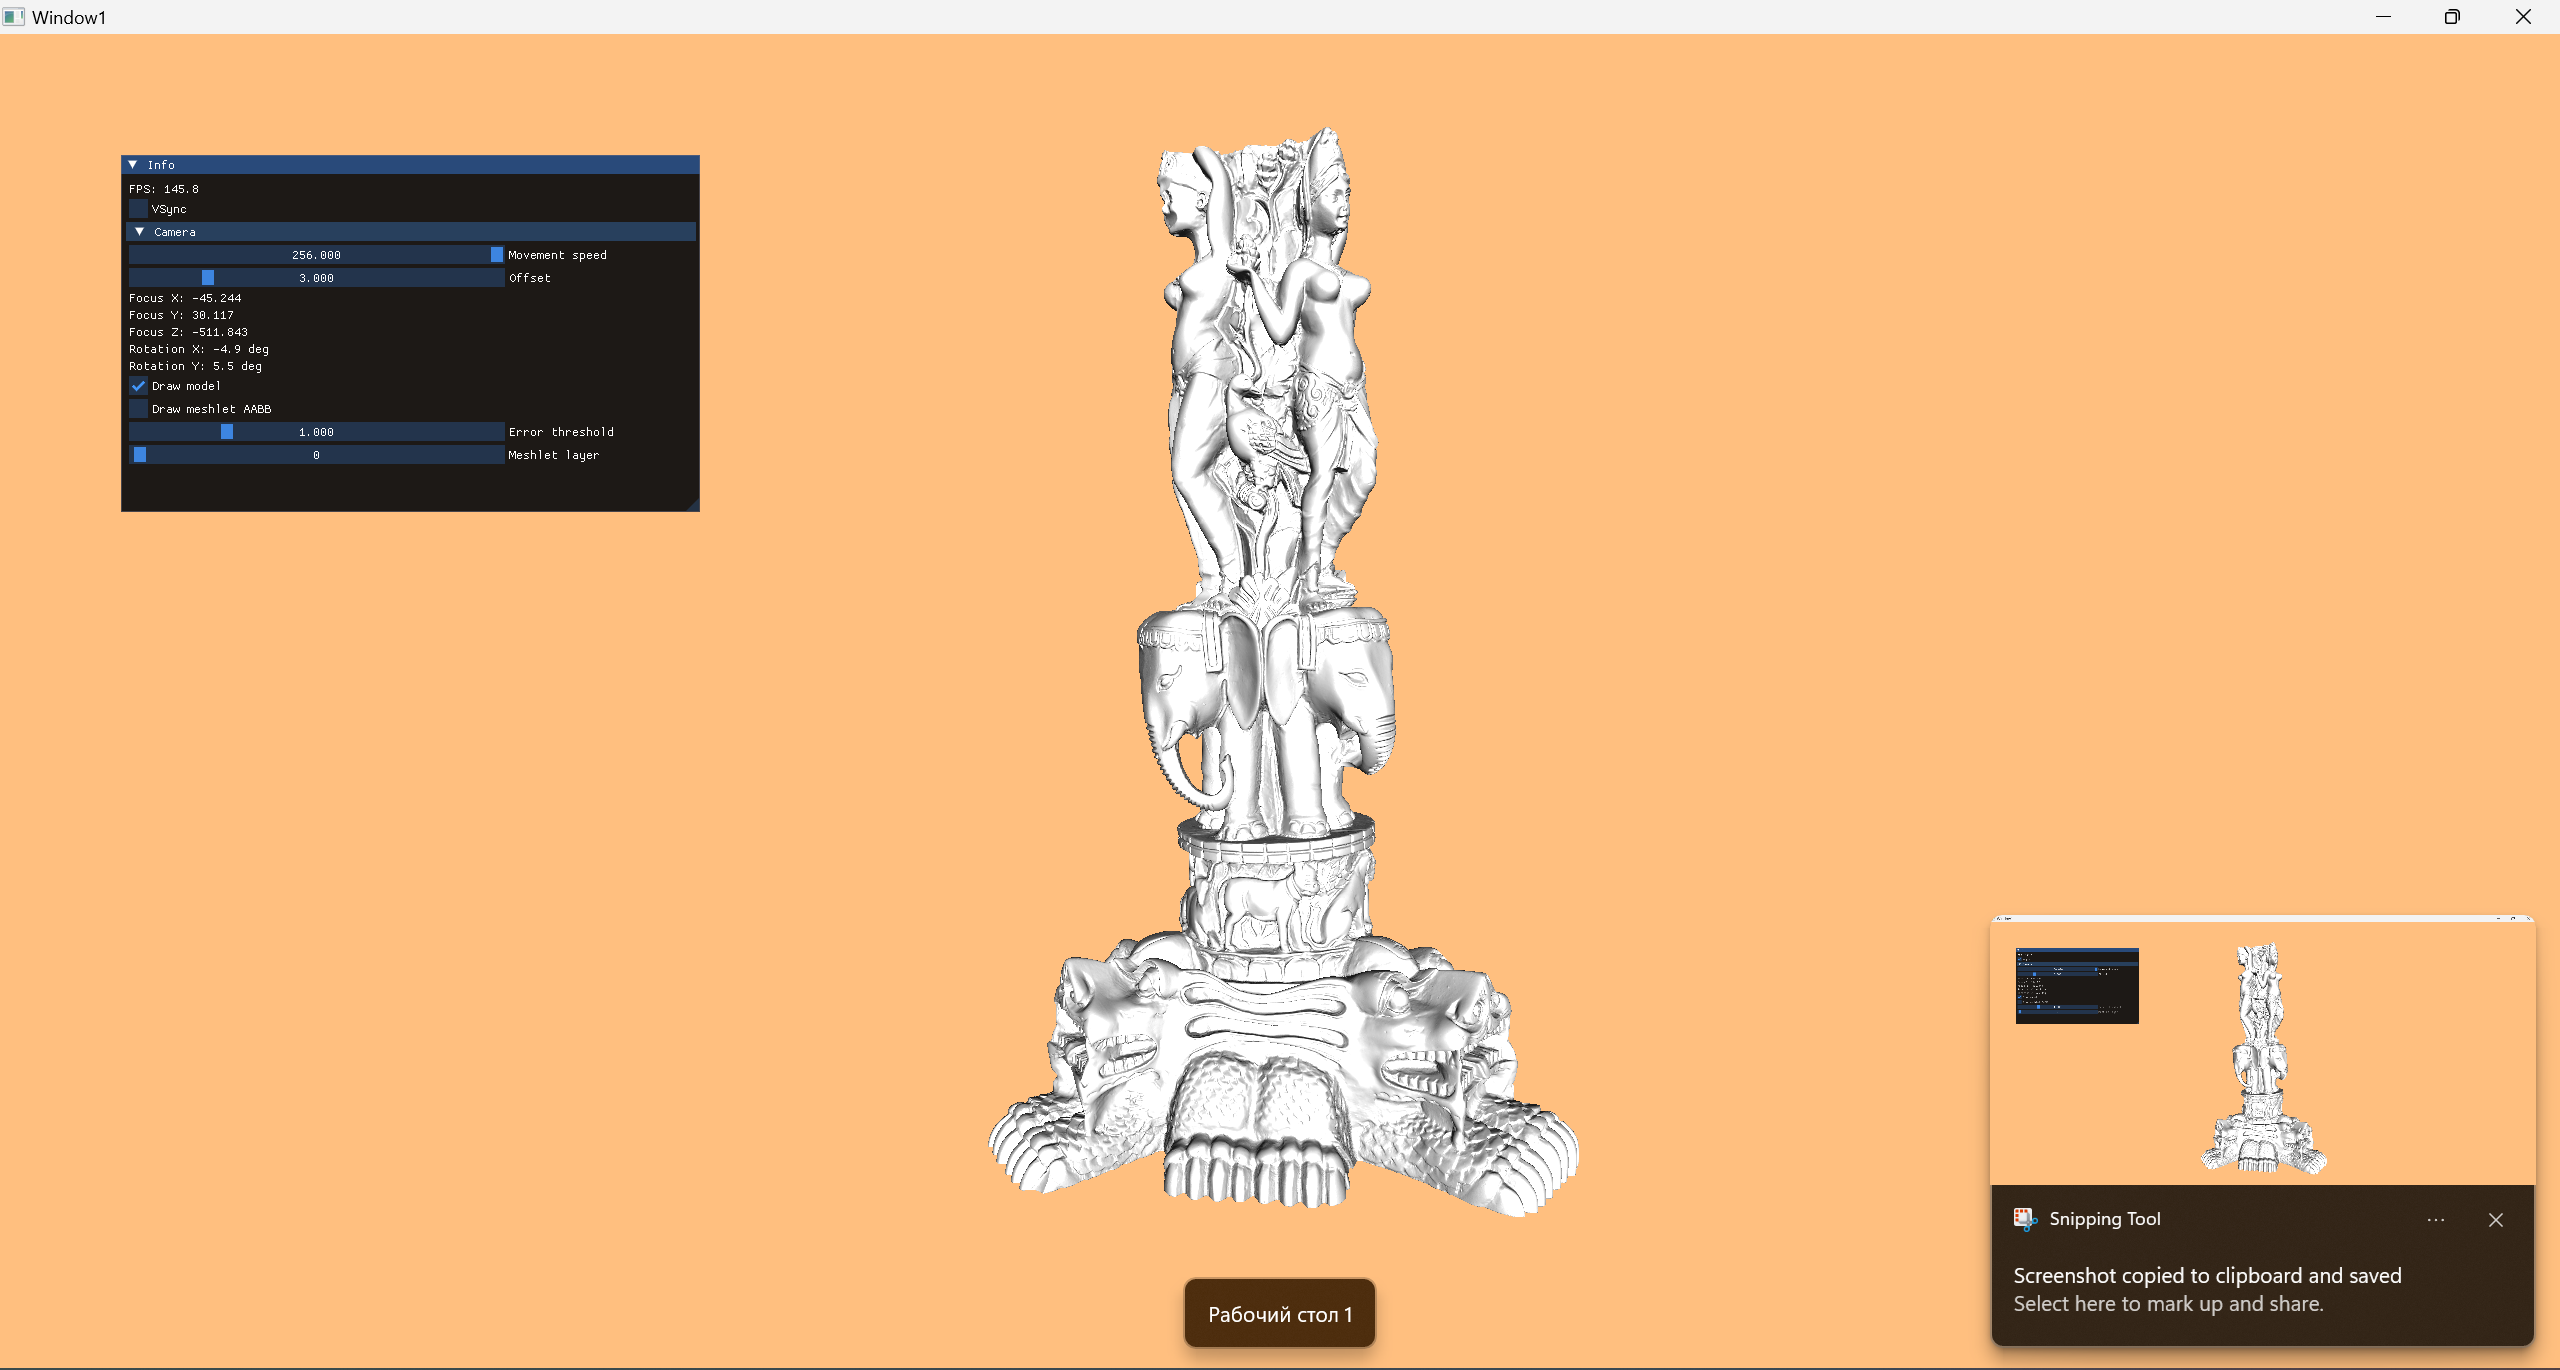
\includegraphics[width=\textwidth]{demo-0.png}
    \end{frame}

    \begin{frame}{Реализация}
        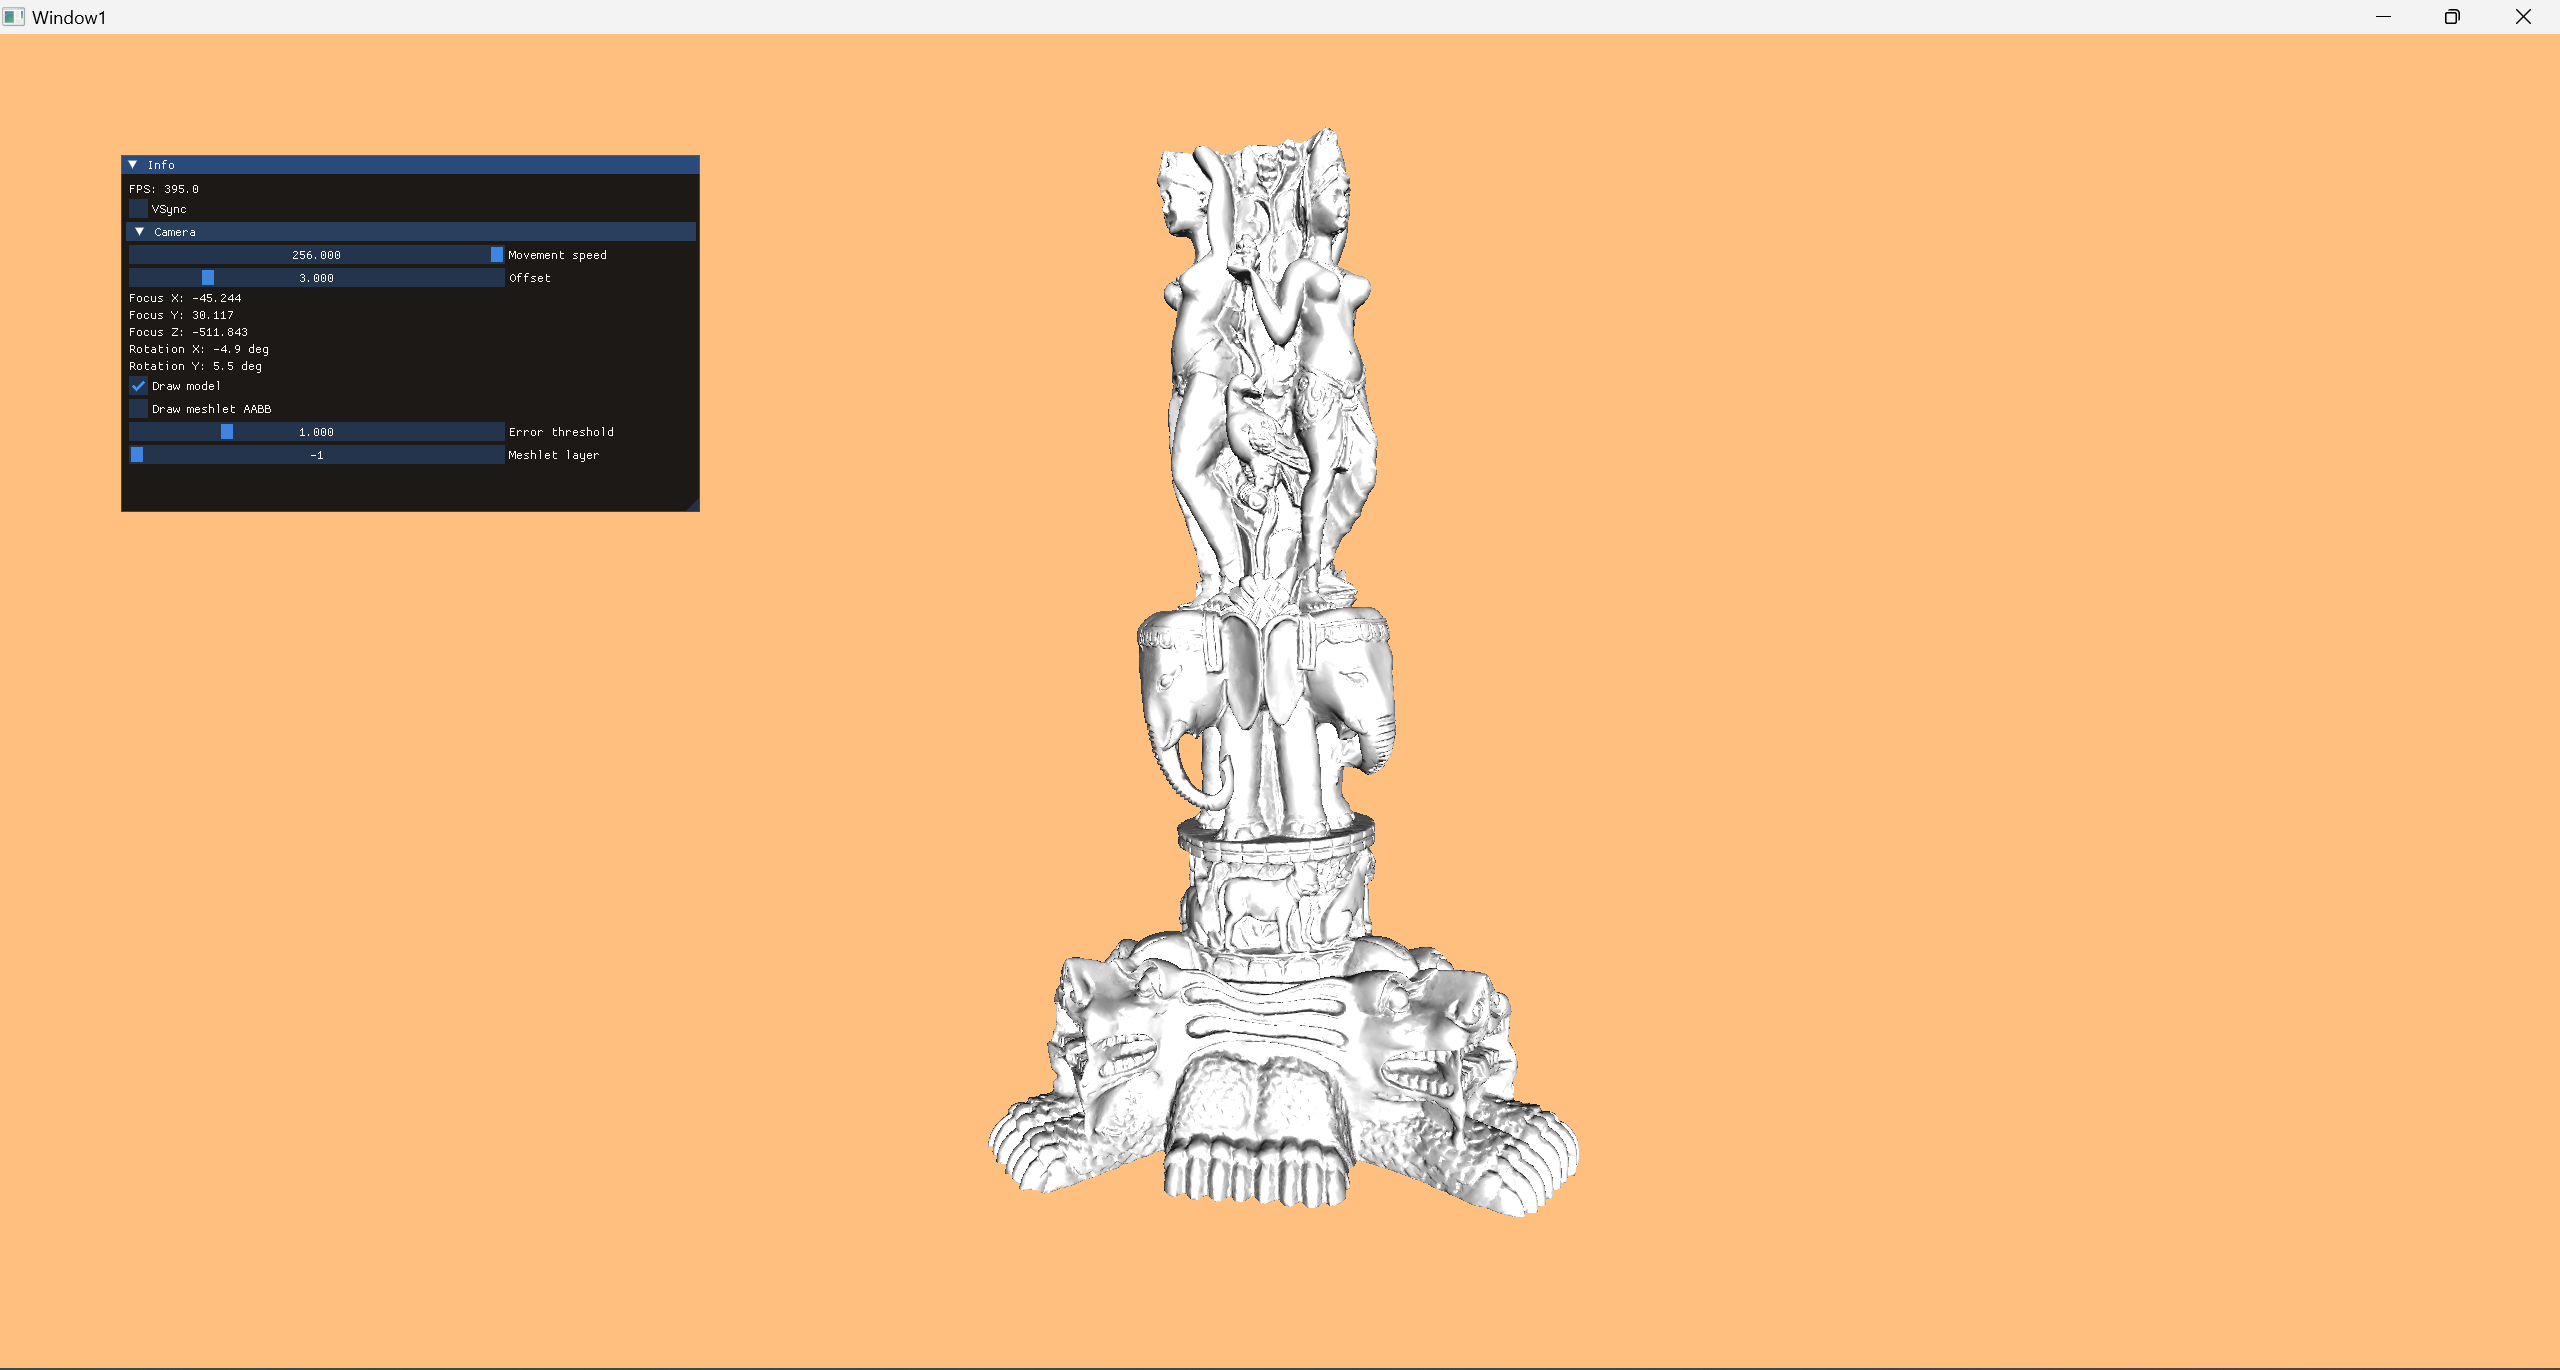
\includegraphics[width=\textwidth]{demo-1.png}
    \end{frame}

    \begin{frame}{Реализация}
        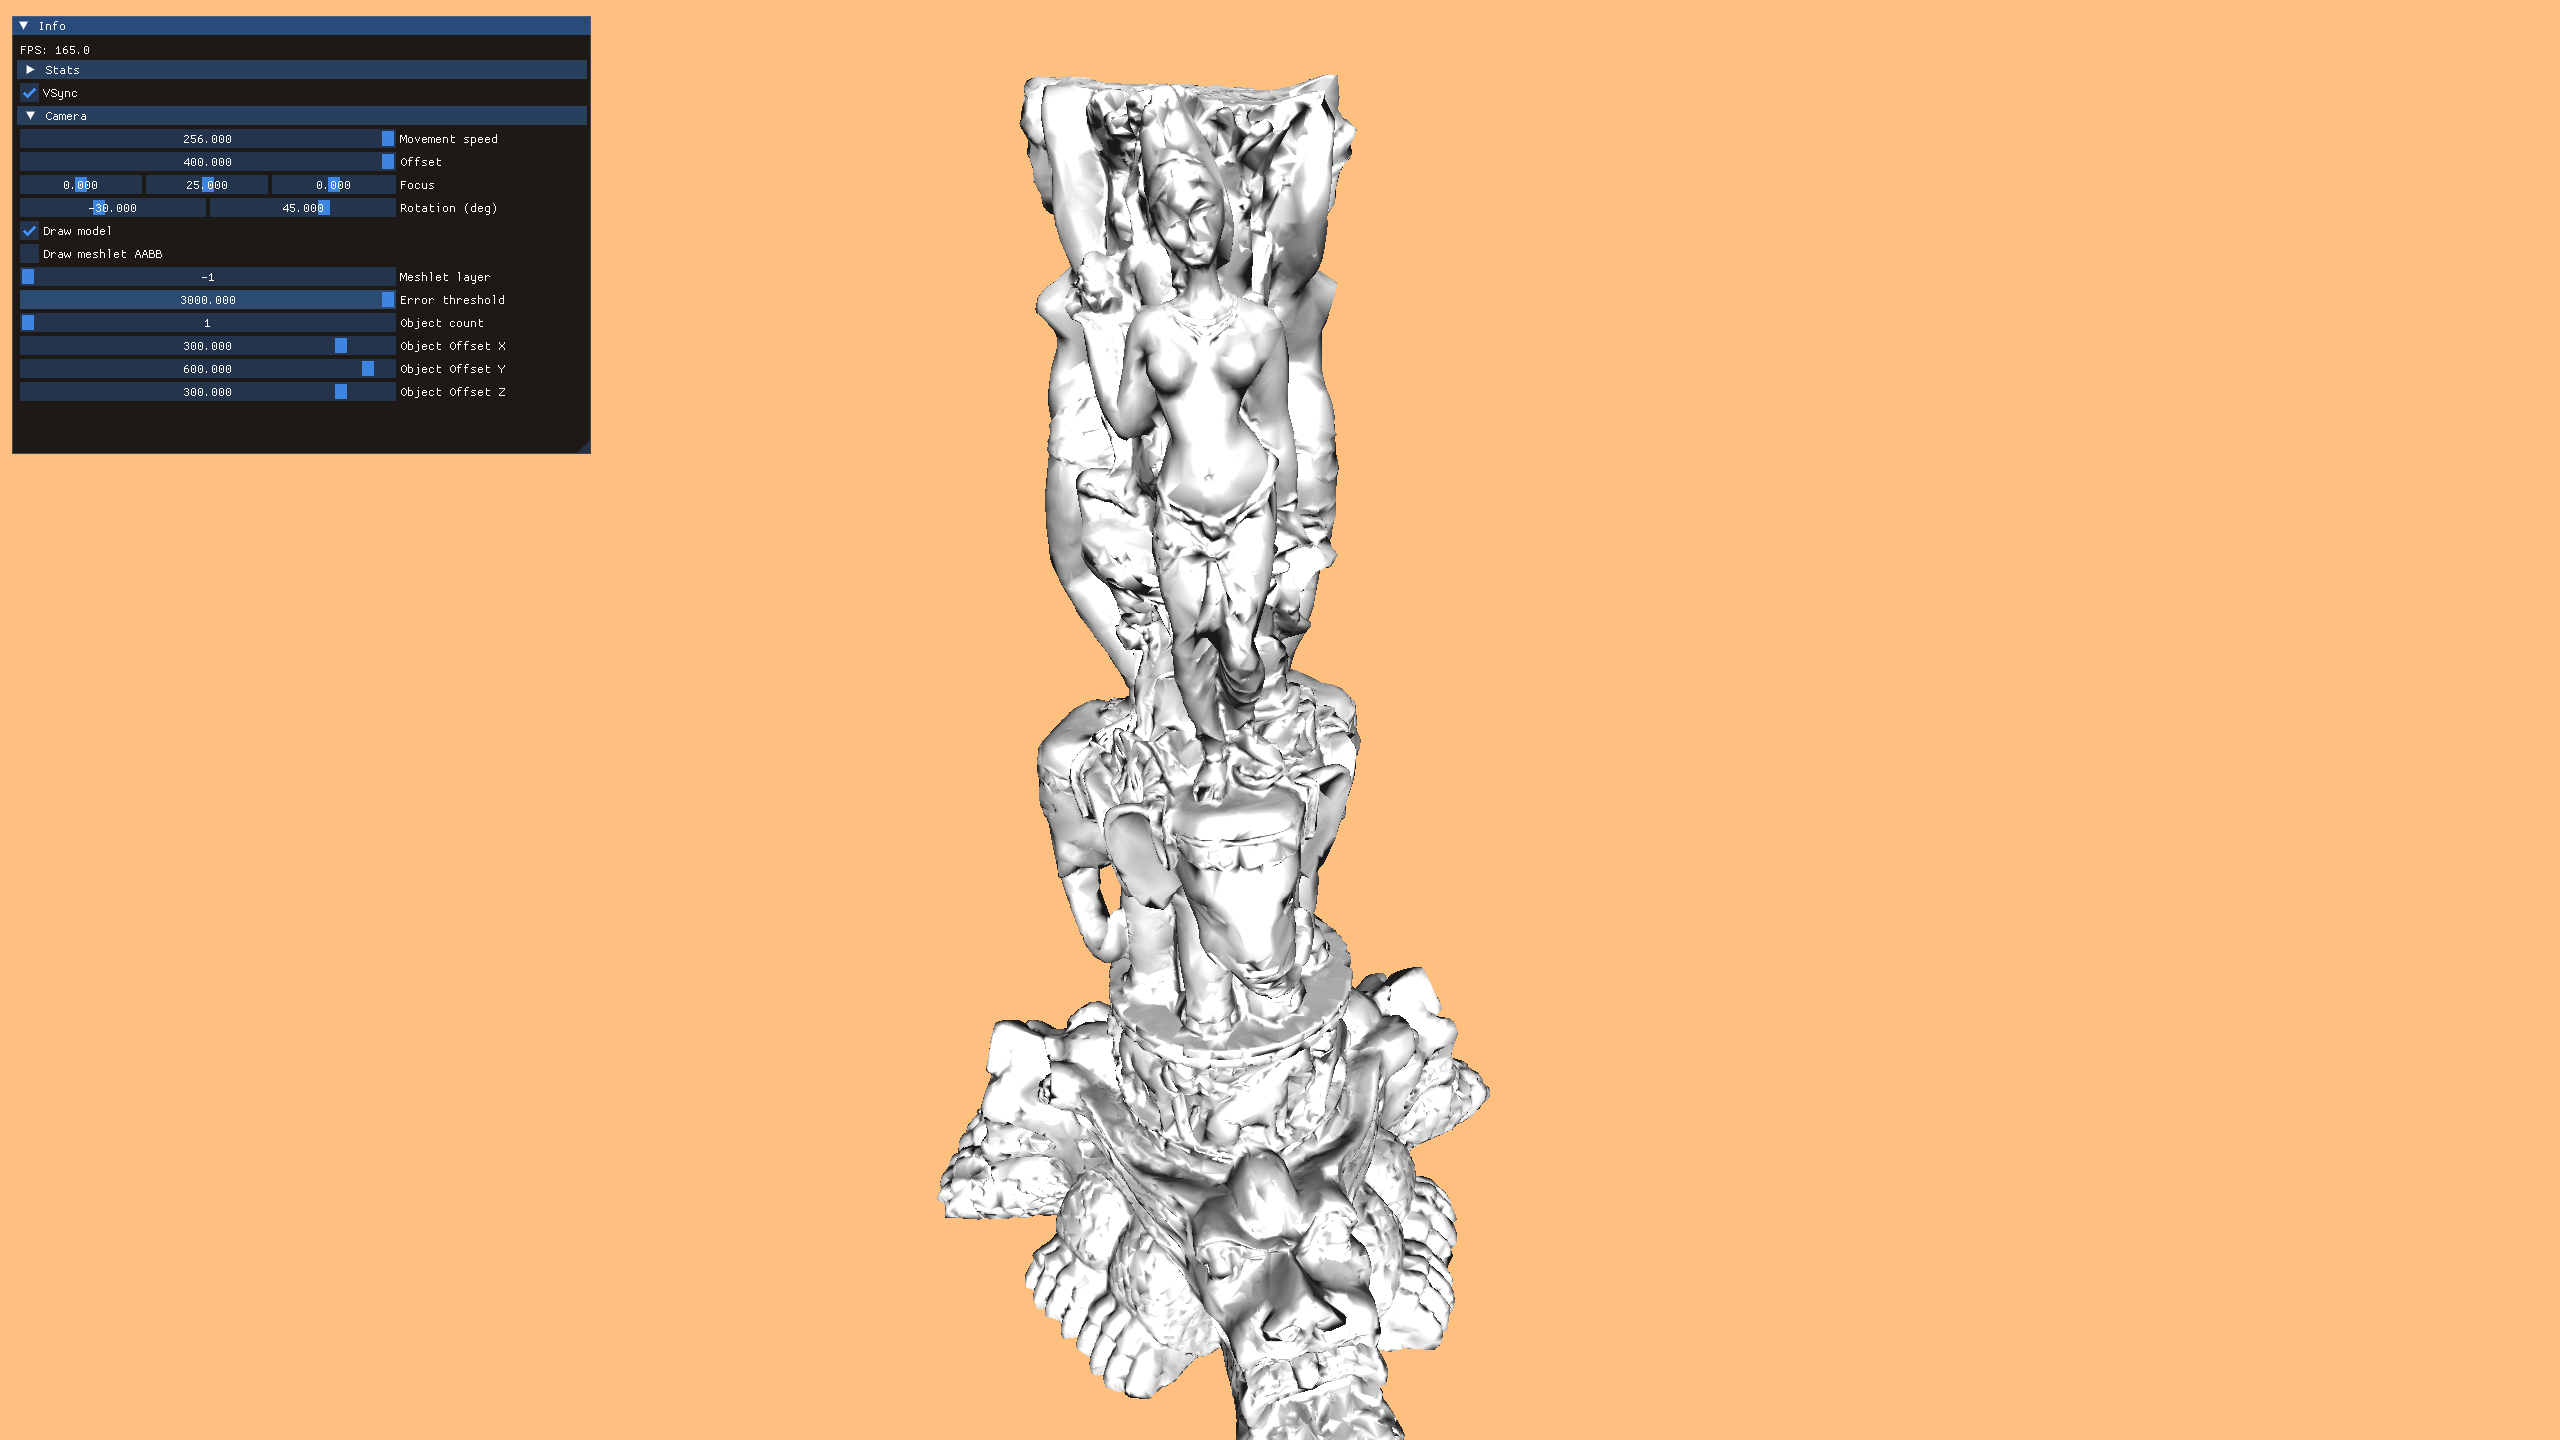
\includegraphics[width=\textwidth]{demo-2.png}
    \end{frame}

    \begin{frame}{Проблемы при реализации}
        \begin{itemize}
            \item Разбиение на мешлеты --- NP-трудная задача
            \item Из-за этого алгоритмы --- приближения
            \item Ограничение размера мешлета
        \end{itemize}
    \end{frame}

    \begin{frame}{Проблемы при реализации: мешлеты}
        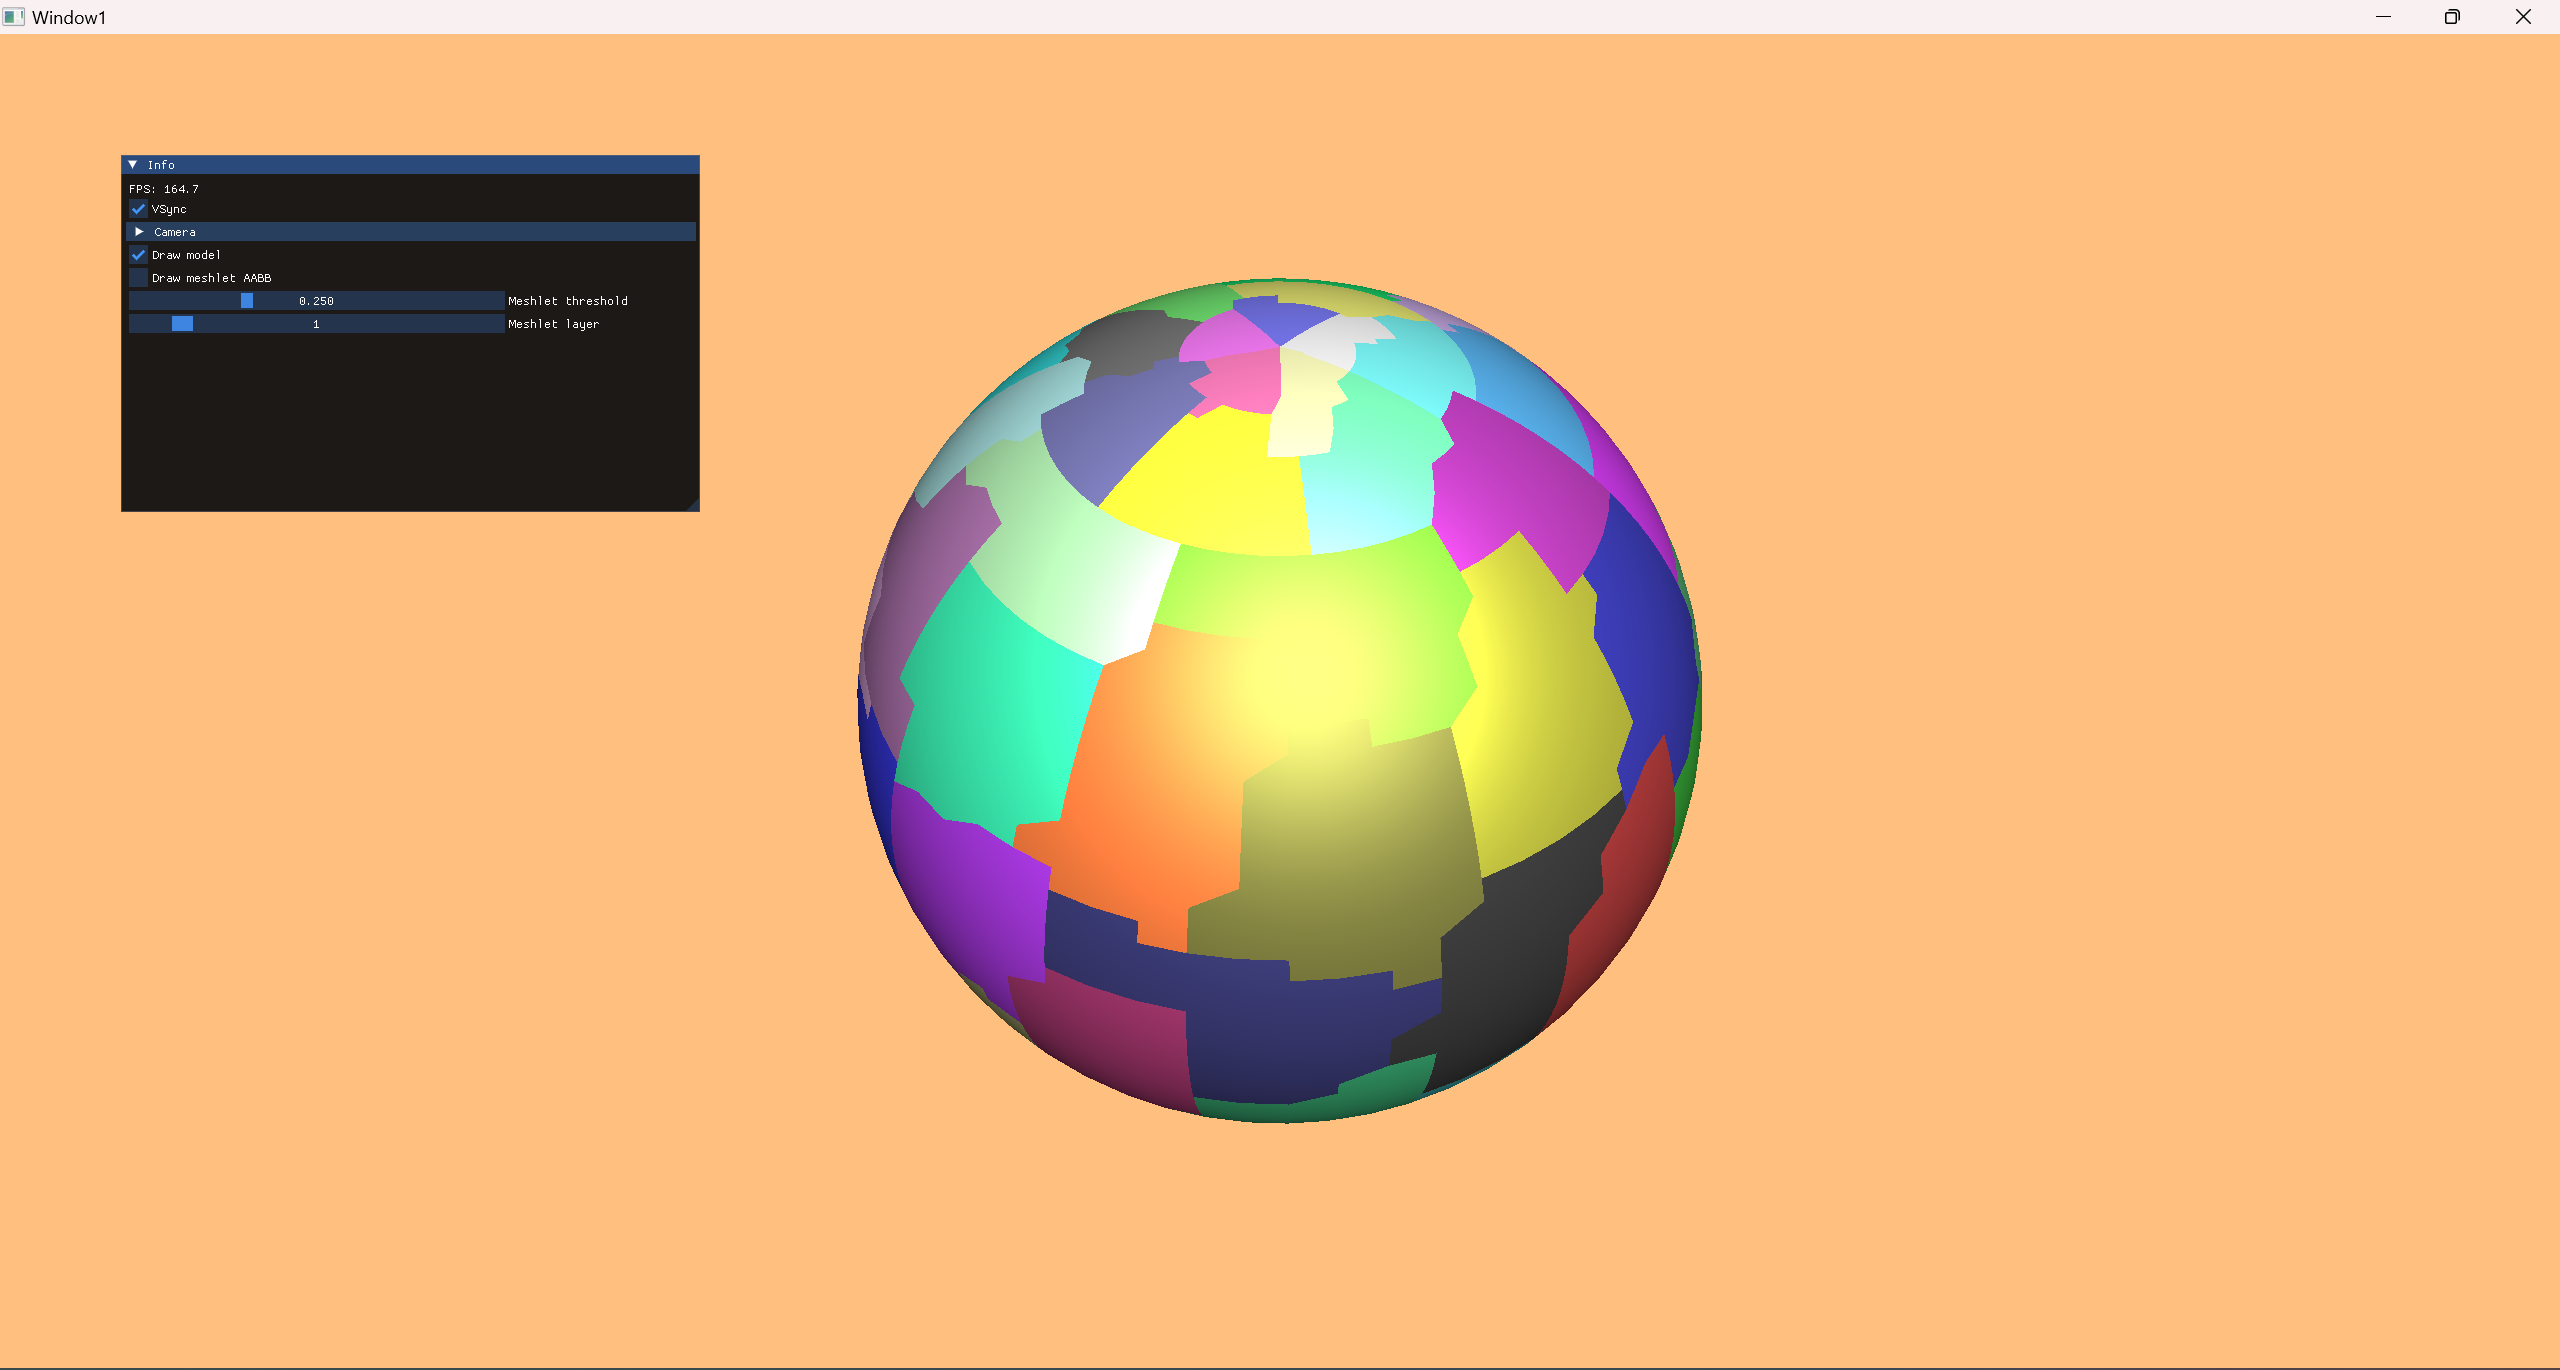
\includegraphics[width=\textwidth]{sphere0.png}
    \end{frame}

    \begin{frame}{Проблемы при реализации: последствия}
        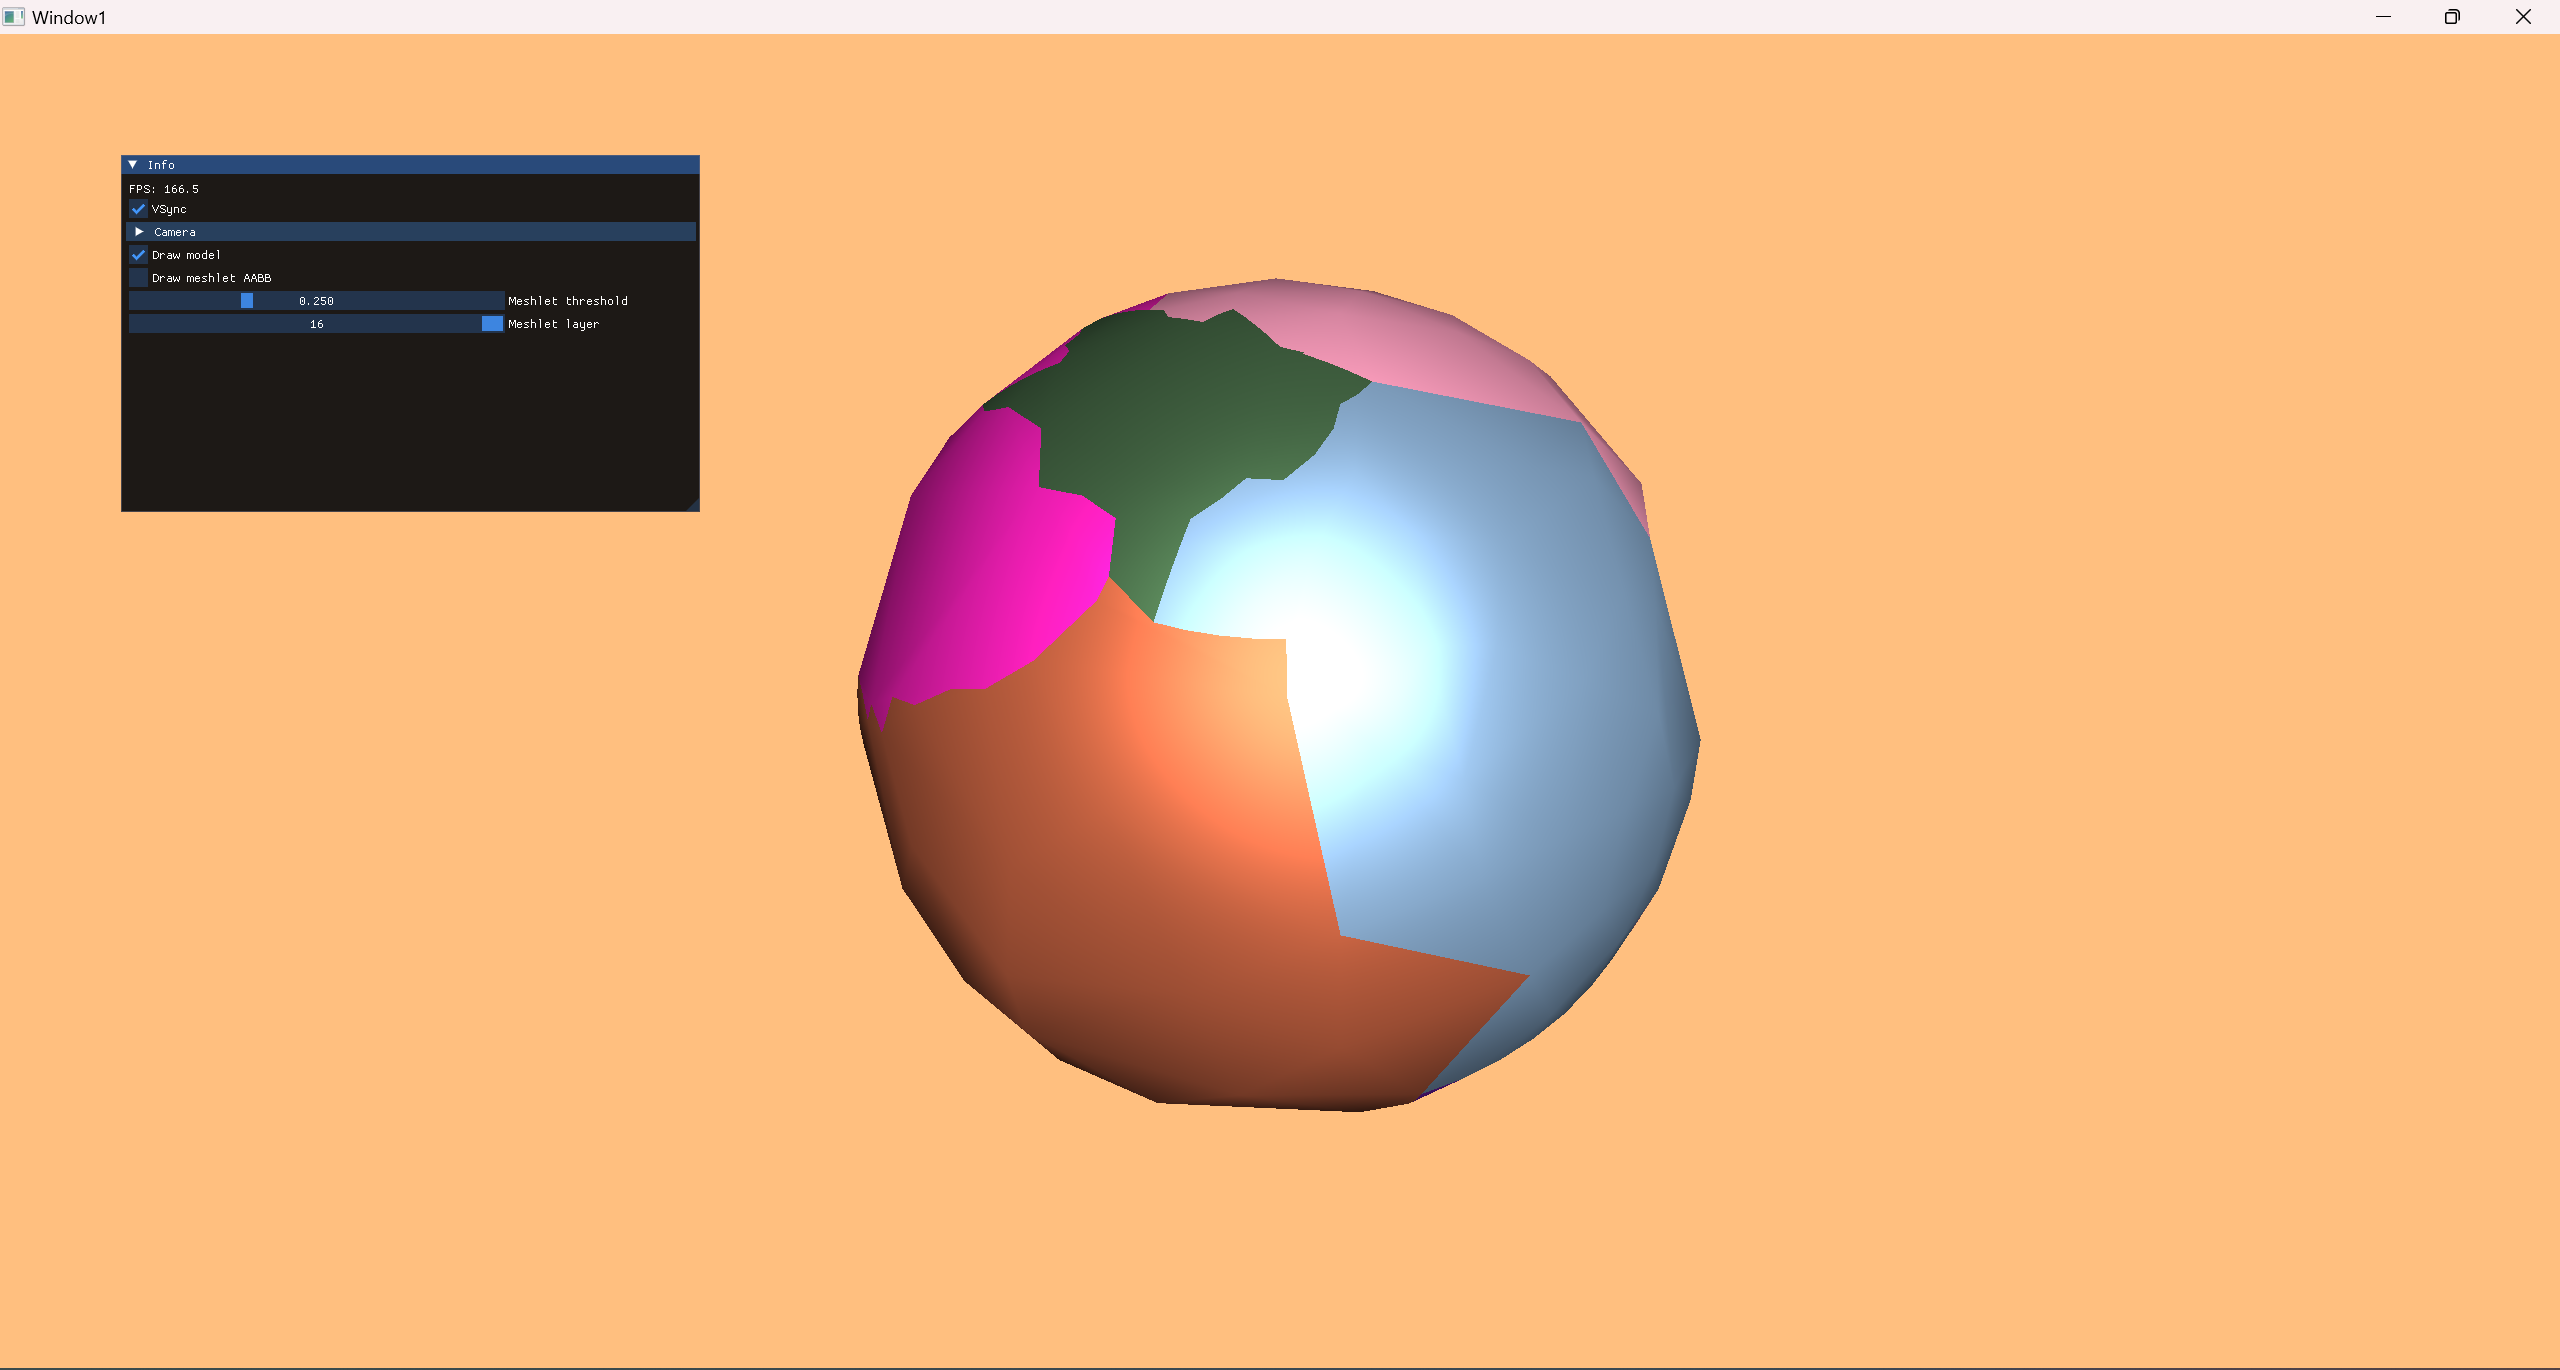
\includegraphics[width=\textwidth]{sphere1.png}
    \end{frame}

    \begin{frame}{Принципиальные ограничения}
        \begin{itemize}
            \item Оценка искажения не зависит от направления
            \item Невозможна анимация
            \item Некоторые меши так не сжимаются
        \end{itemize}
    \end{frame}

    \begin{frame}{Принципиальное ограничение: объём}
        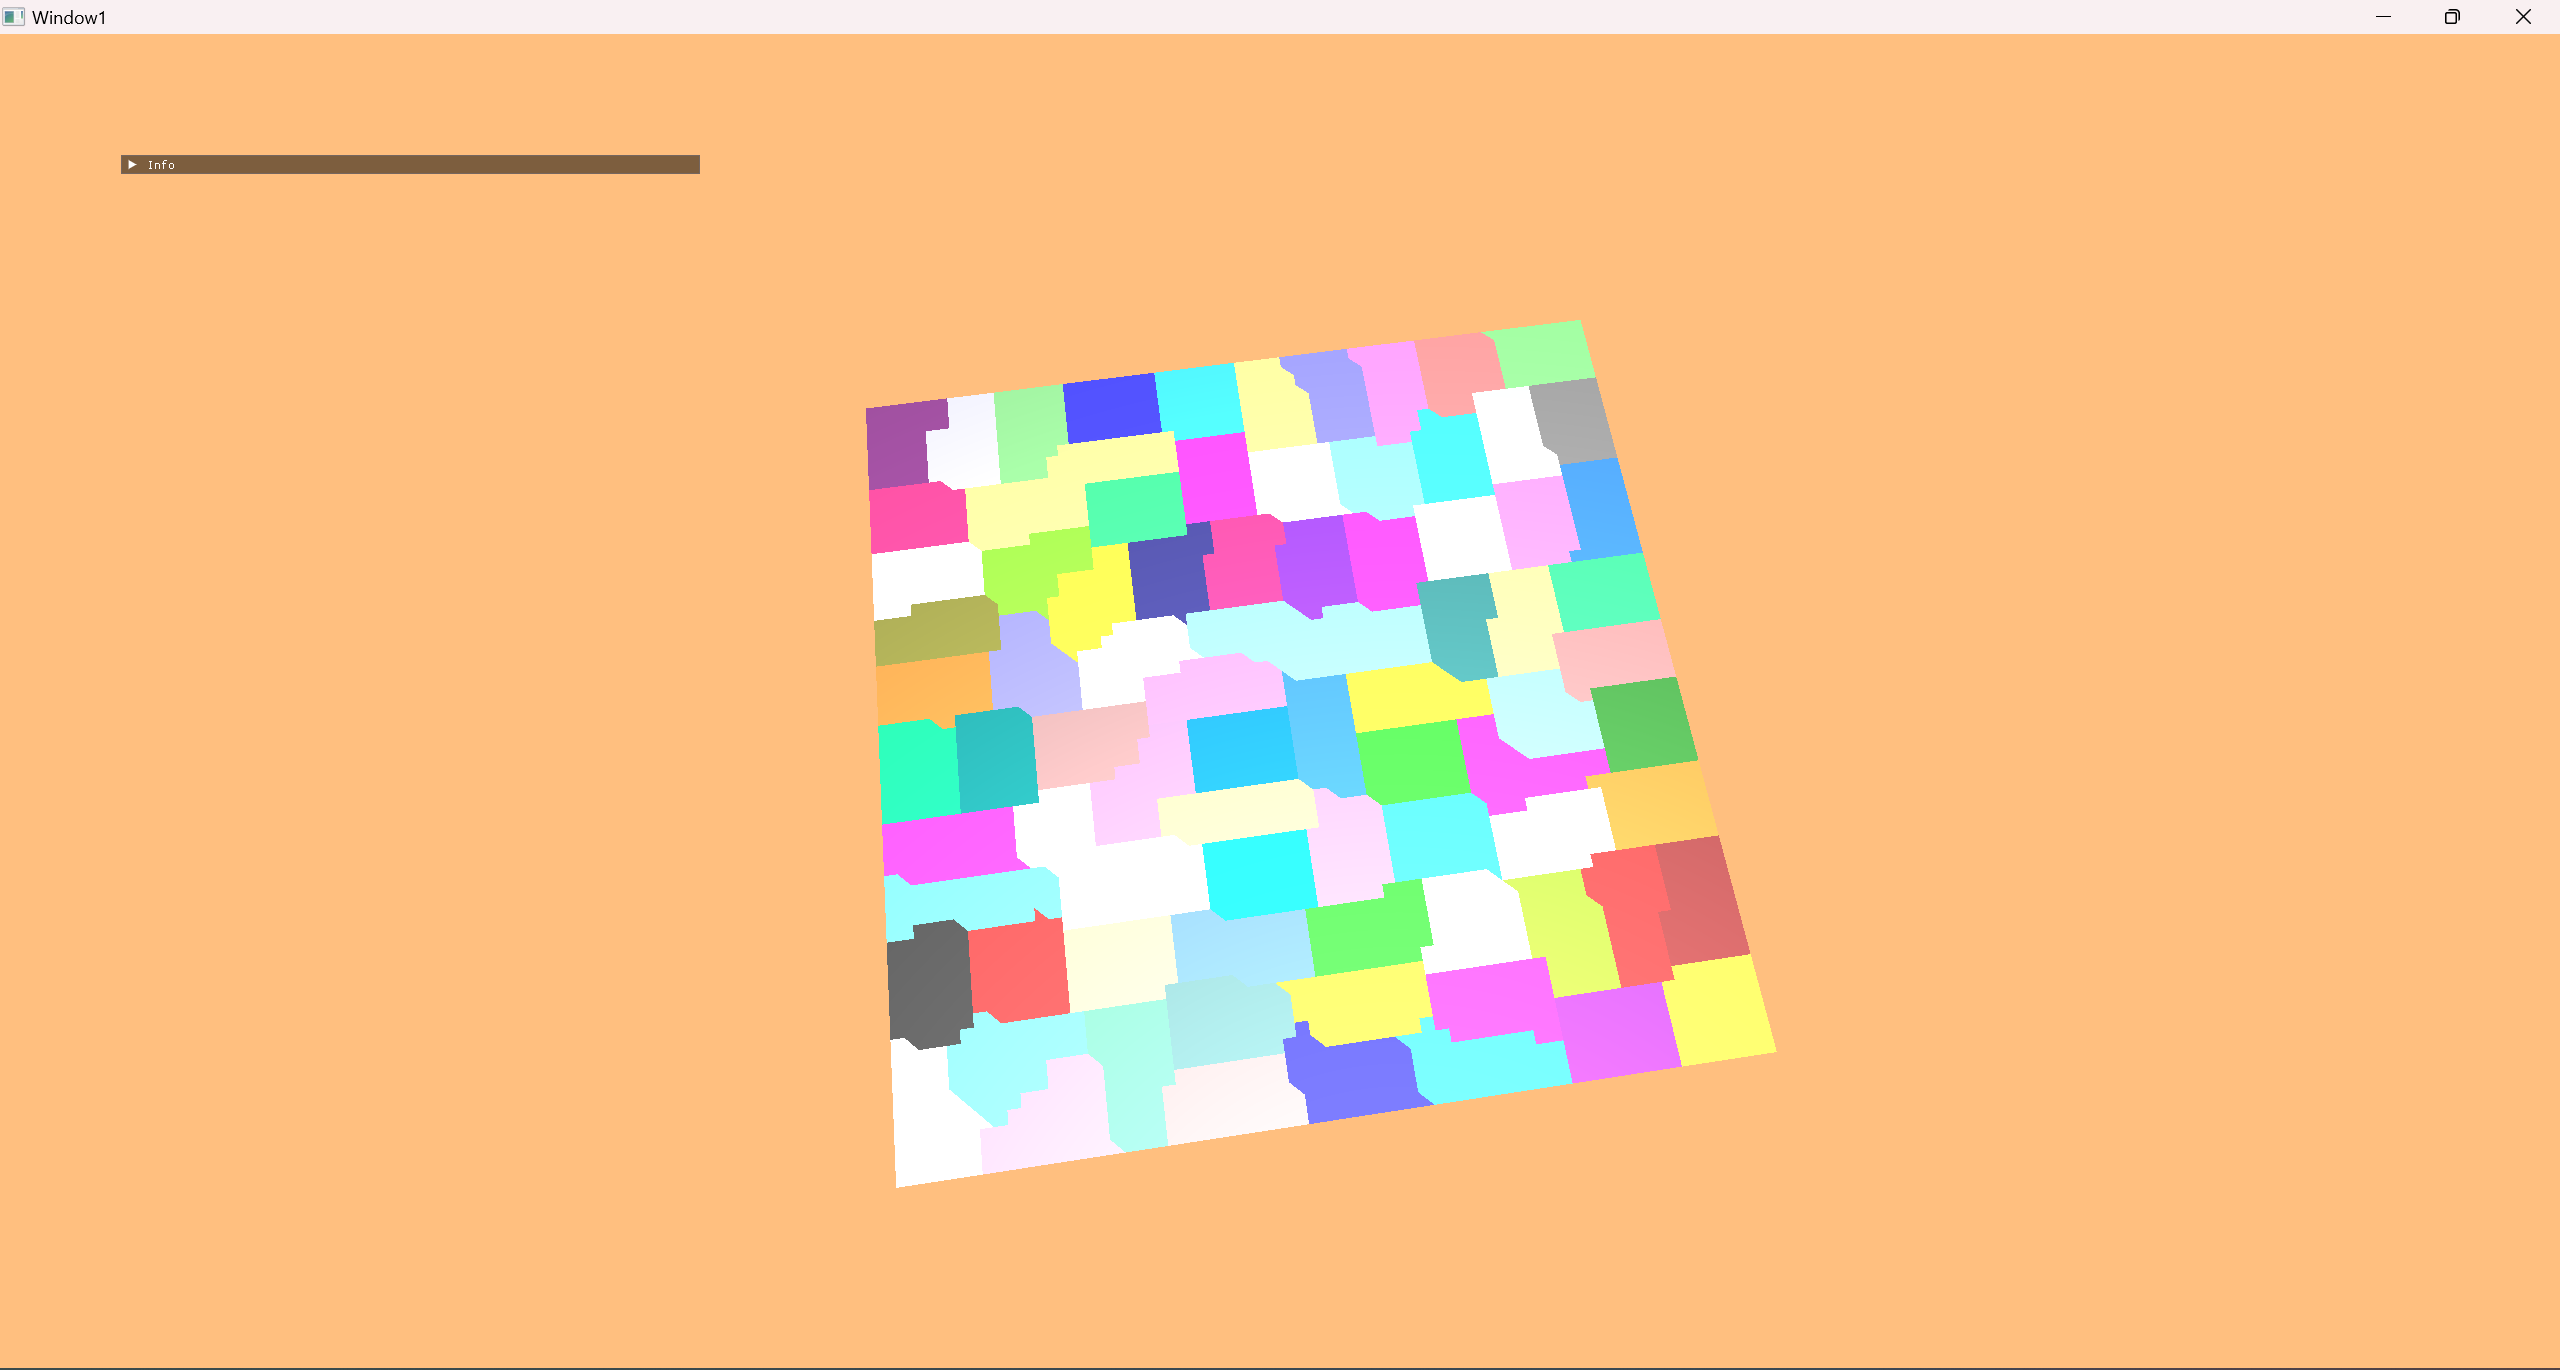
\includegraphics[width=\textwidth]{plane0.png}
    \end{frame}

    \begin{frame}{Принципиальное ограничение: объём}
        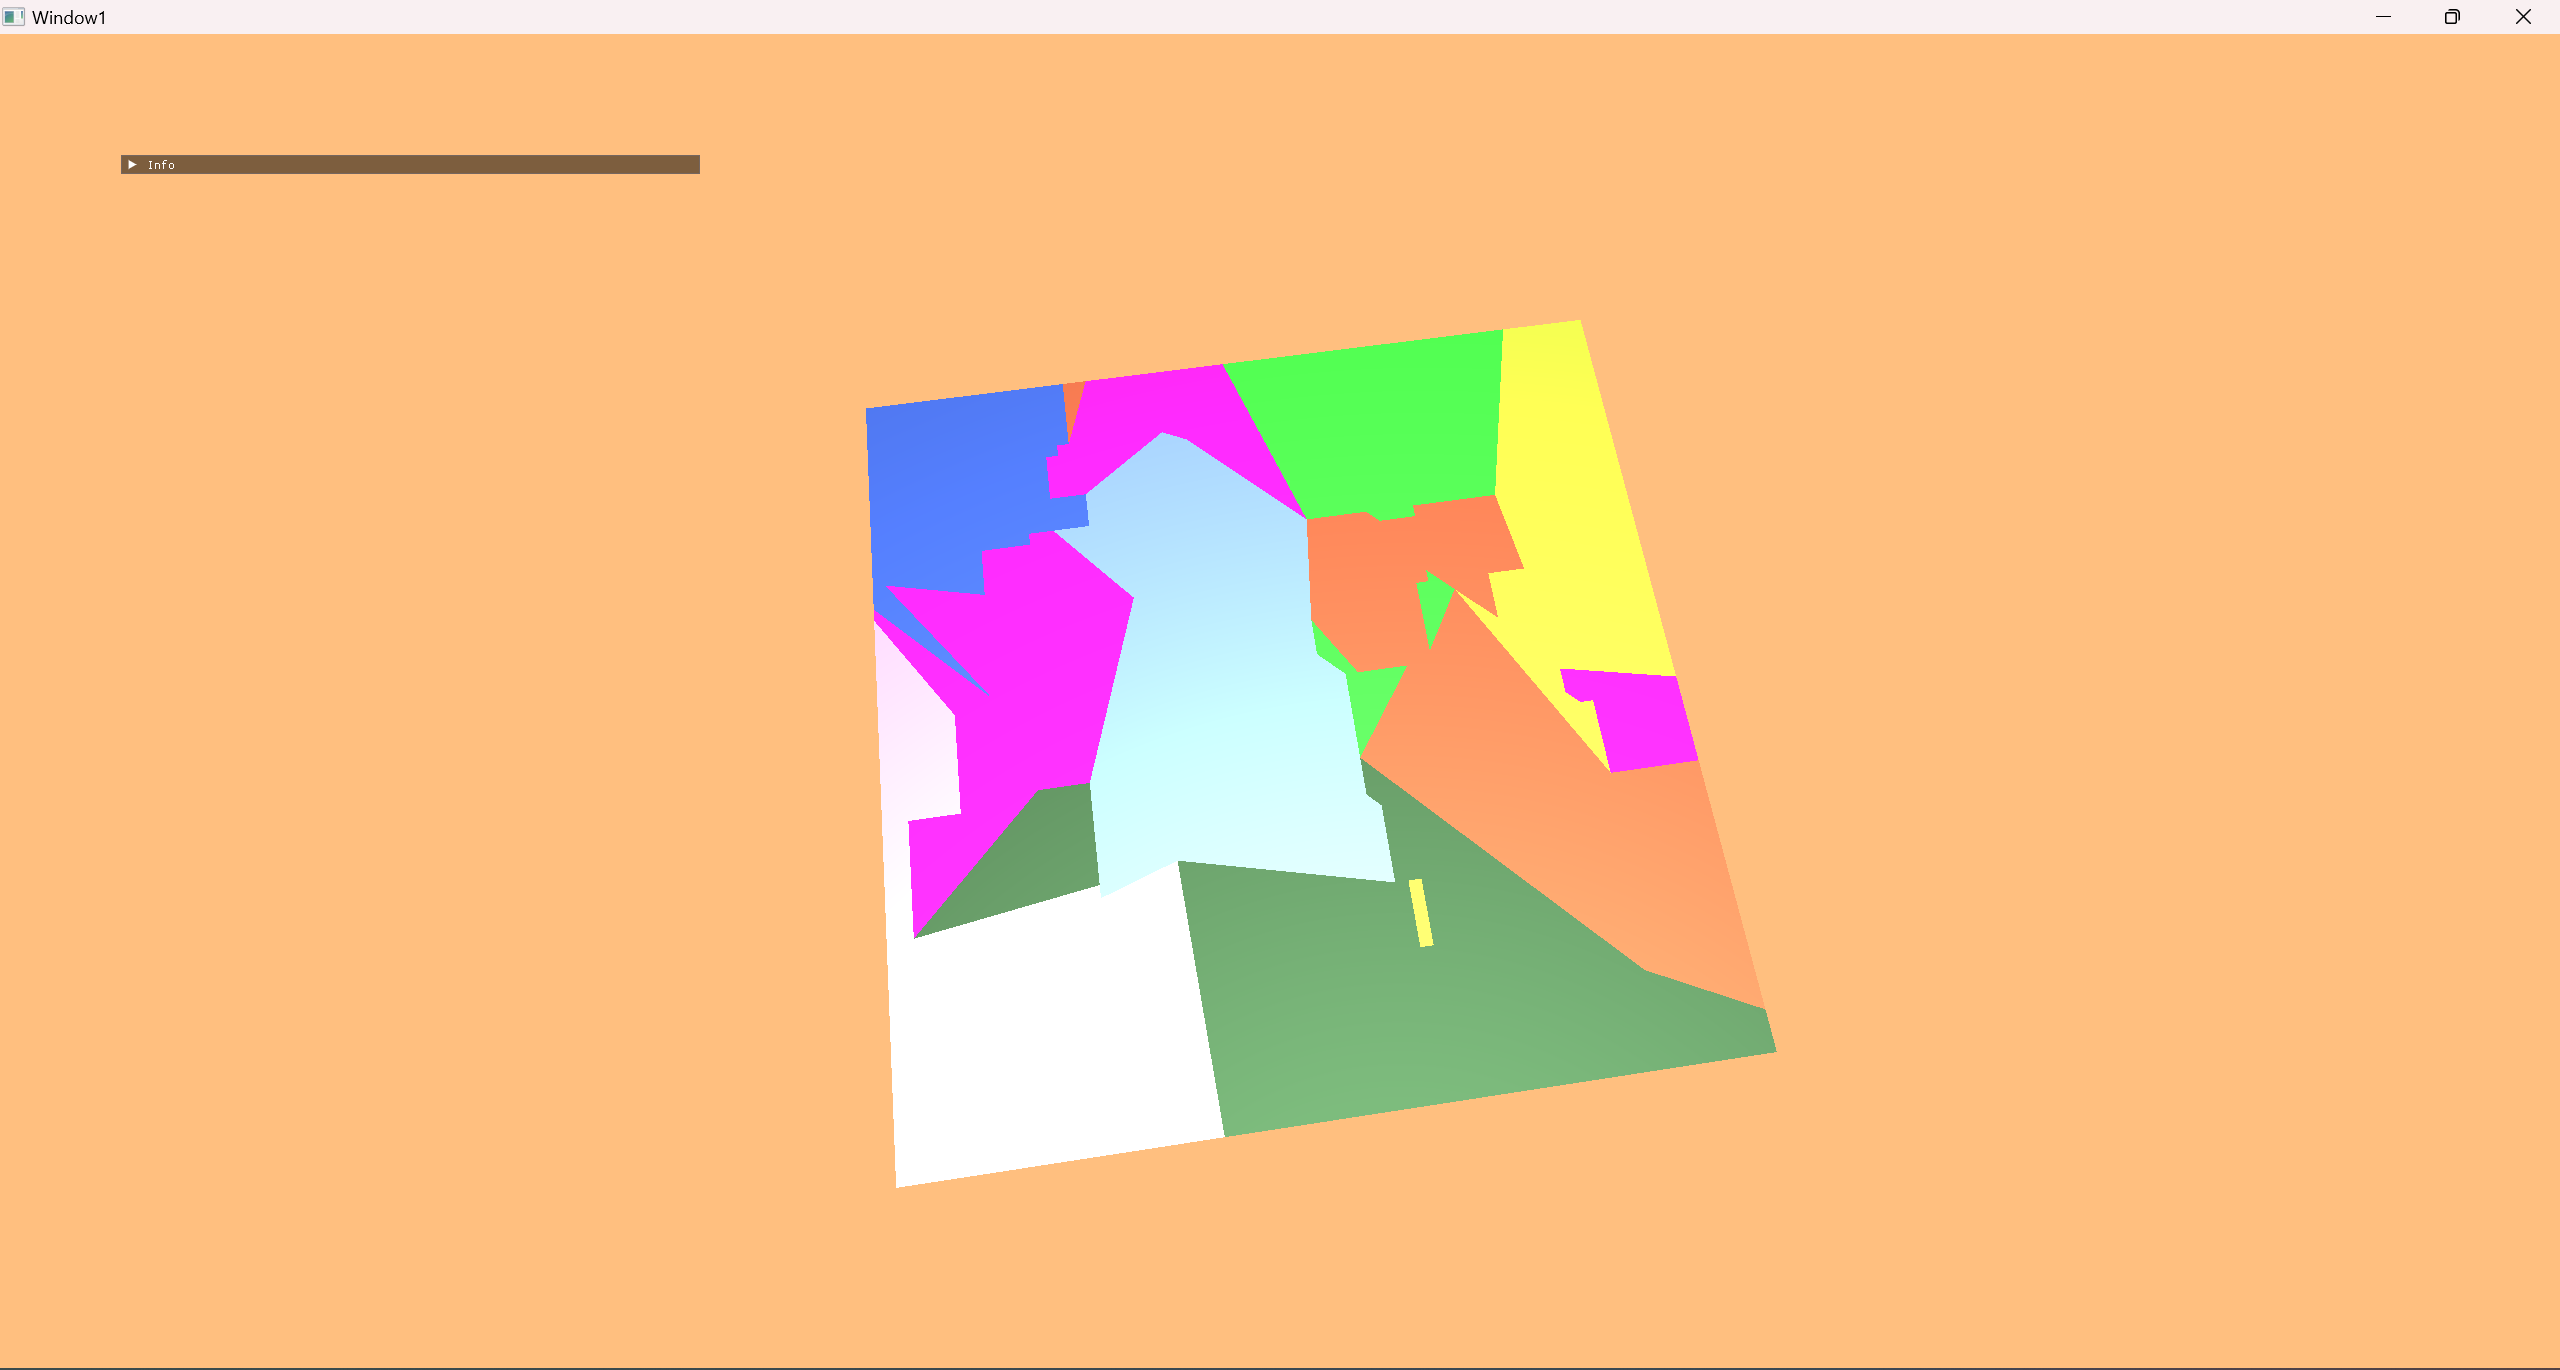
\includegraphics[width=\textwidth]{plane1.png}
    \end{frame}

    % \begin{frame}{Сравнение с некластерной детализацией}
    %     Пока не проводилось
    % \end{frame}

    \begin{frame}{Результаты}
        \begin{itemize}
            \item Выявлены существенные проблемы, которые надо решать в полной реализации
            \item Выявлены принципиальные ограничения технологии
            \item Получена реализация для объяснимых замеров
        \end{itemize}
    \end{frame}
\end{document}
